% \iffalse
\let\negmedspace\undefined
\let\negthickspace\undefined
\documentclass[journal,12pt,twocolumn]{IEEEtran}
\usepackage{cite}
\usepackage{amsmath,amssymb,amsfonts,amsthm}
\usepackage{algorithmic}
\usepackage{graphicx}
\usepackage{textcomp}
\usepackage{xcolor}
\usepackage{txfonts}
\usepackage{listings}
\usepackage{enumitem}
\usepackage{mathtools}
\usepackage{gensymb}
\usepackage{comment}
\usepackage[breaklinks=true]{hyperref}
\usepackage{tkz-euclide} 
\usepackage{listings}
\usepackage{gvv}                                        
\def\inputGnumericTable{}                                 
\usepackage[latin1]{inputenc}                                
\usepackage{color}                                            
\usepackage{array}                                            
\usepackage{longtable}                                       
\usepackage{calc}                                             
\usepackage{multirow}                                         
\usepackage{hhline}                                           
\usepackage{ifthen}                                           
\usepackage{lscape}
\newtheorem{theorem}{Theorem}[section]
\newtheorem{problem}{Problem}
\newtheorem{proposition}{Proposition}[section]
\newtheorem{lemma}{Lemma}[section]
\newtheorem{corollary}[theorem]{Corollary}
\newtheorem{example}{Example}[section]
\newtheorem{definition}[problem]{Definition}
\newcommand{\BEQA}{\begin{eqnarray}}
\newcommand{\EEQA}{\end{eqnarray}}
\newcommand{\define}{\stackrel{\triangle}{=}}
\theoremstyle{remark}
\newtheorem{rem}{Remark}
\begin{document}

\bibliographystyle{IEEEtran}
\vspace{3cm}

\title{NCERT 11.9.3.Q10}
\author{EE23BTECH11224 - Sri Krishna Prabhas Yadla$^{*}$% <-this % stops a space
}
\maketitle
\newpage
\bigskip

\renewcommand{\thefigure}{\arabic{figure}}
\renewcommand{\thetable}{\arabic{table}}


\vspace{3cm}
\textbf{Question:} Find the sum to indicated number of terms in the geometric progression $x^3,x^5,x^7,...n$ terms (if $x\neq\pm1$).
\\
\solution
% \fi
\begin{table}[htbp]
\centering
\def\arraystrech{1.5}
	\begin{tabular}{|p{2.5cm}|p{1.5cm}|p{3cm}|}
\hline
		\textbf{Input Parameters} & \textbf{Values} & \textbf{Description} \\
\hline
		$x(0)$ & $x^3$ & Initial term\\
\hline
		$r$ & $x^2$ & Common ratio\\
\hline
\end{tabular}
\caption{Given inputs}
\label{tab:1.11.9.3.Q10}
\end{table}

\newline
From \tabref{tab:1.11.9.3.Q10}
\begin{align}
	X(z) &= \frac{x(0)}{1-rz^{-1}} \\
	&= \frac{x^3}{1-x^2z^{-1}} \quad \abs{z}>x^2 \\
	y(n) &= x(n) * u(n) \\
	Y(z) &= X(z)U(z) \\
	&= \frac{x^3}{(1-x^2z^{-1})(1-z^{-1})} \quad  \abs{z} > x^2 \cap \abs{z}>1\\
	&= \frac{x^3}{x^2-1}\brak{\frac{x^2}{1-x^2z^{-1}}-\frac{1}{1-z^{-1}}} \\
	u(n) &\system{Z} \frac{1}{1-z^{-1}} \\
	x^{2n+2} u(n) &\system{Z} \frac{x^2}{1-x^2z^{-1}}
\end{align}
Taking inverse Z transform of $Y(z)$,
\begin{align}
	y(n) &= x^3\brak{\frac{x^{2n+2}-1}{x^2-1}}u(n)
\end{align}
\begin{figure}[ht!]
	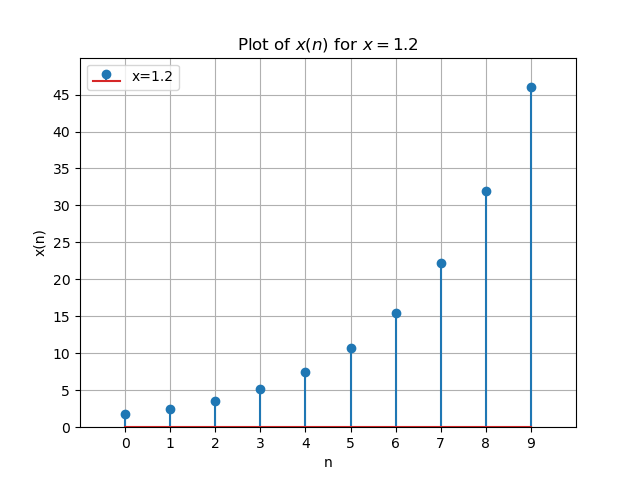
\includegraphics[width=\columnwidth]{figs/plot_2.png}
	\caption{Plot of $x(n)$ for $x=1.2$}
	\label{fig:1.2}
\end{figure}
\end{document}
